\chapter{Bootstrapping Process}
\label{process}

This chapter describes the bootstrapping process in its entirety.
In \autoref{image:process}, we can see the whole process with numerated steps.
We will go through \autoref{image:process} step by step in the following paragraphs to get a better understanding of the whole bootstrapping process.

\begin{figure}[!htbp]
	\centering
	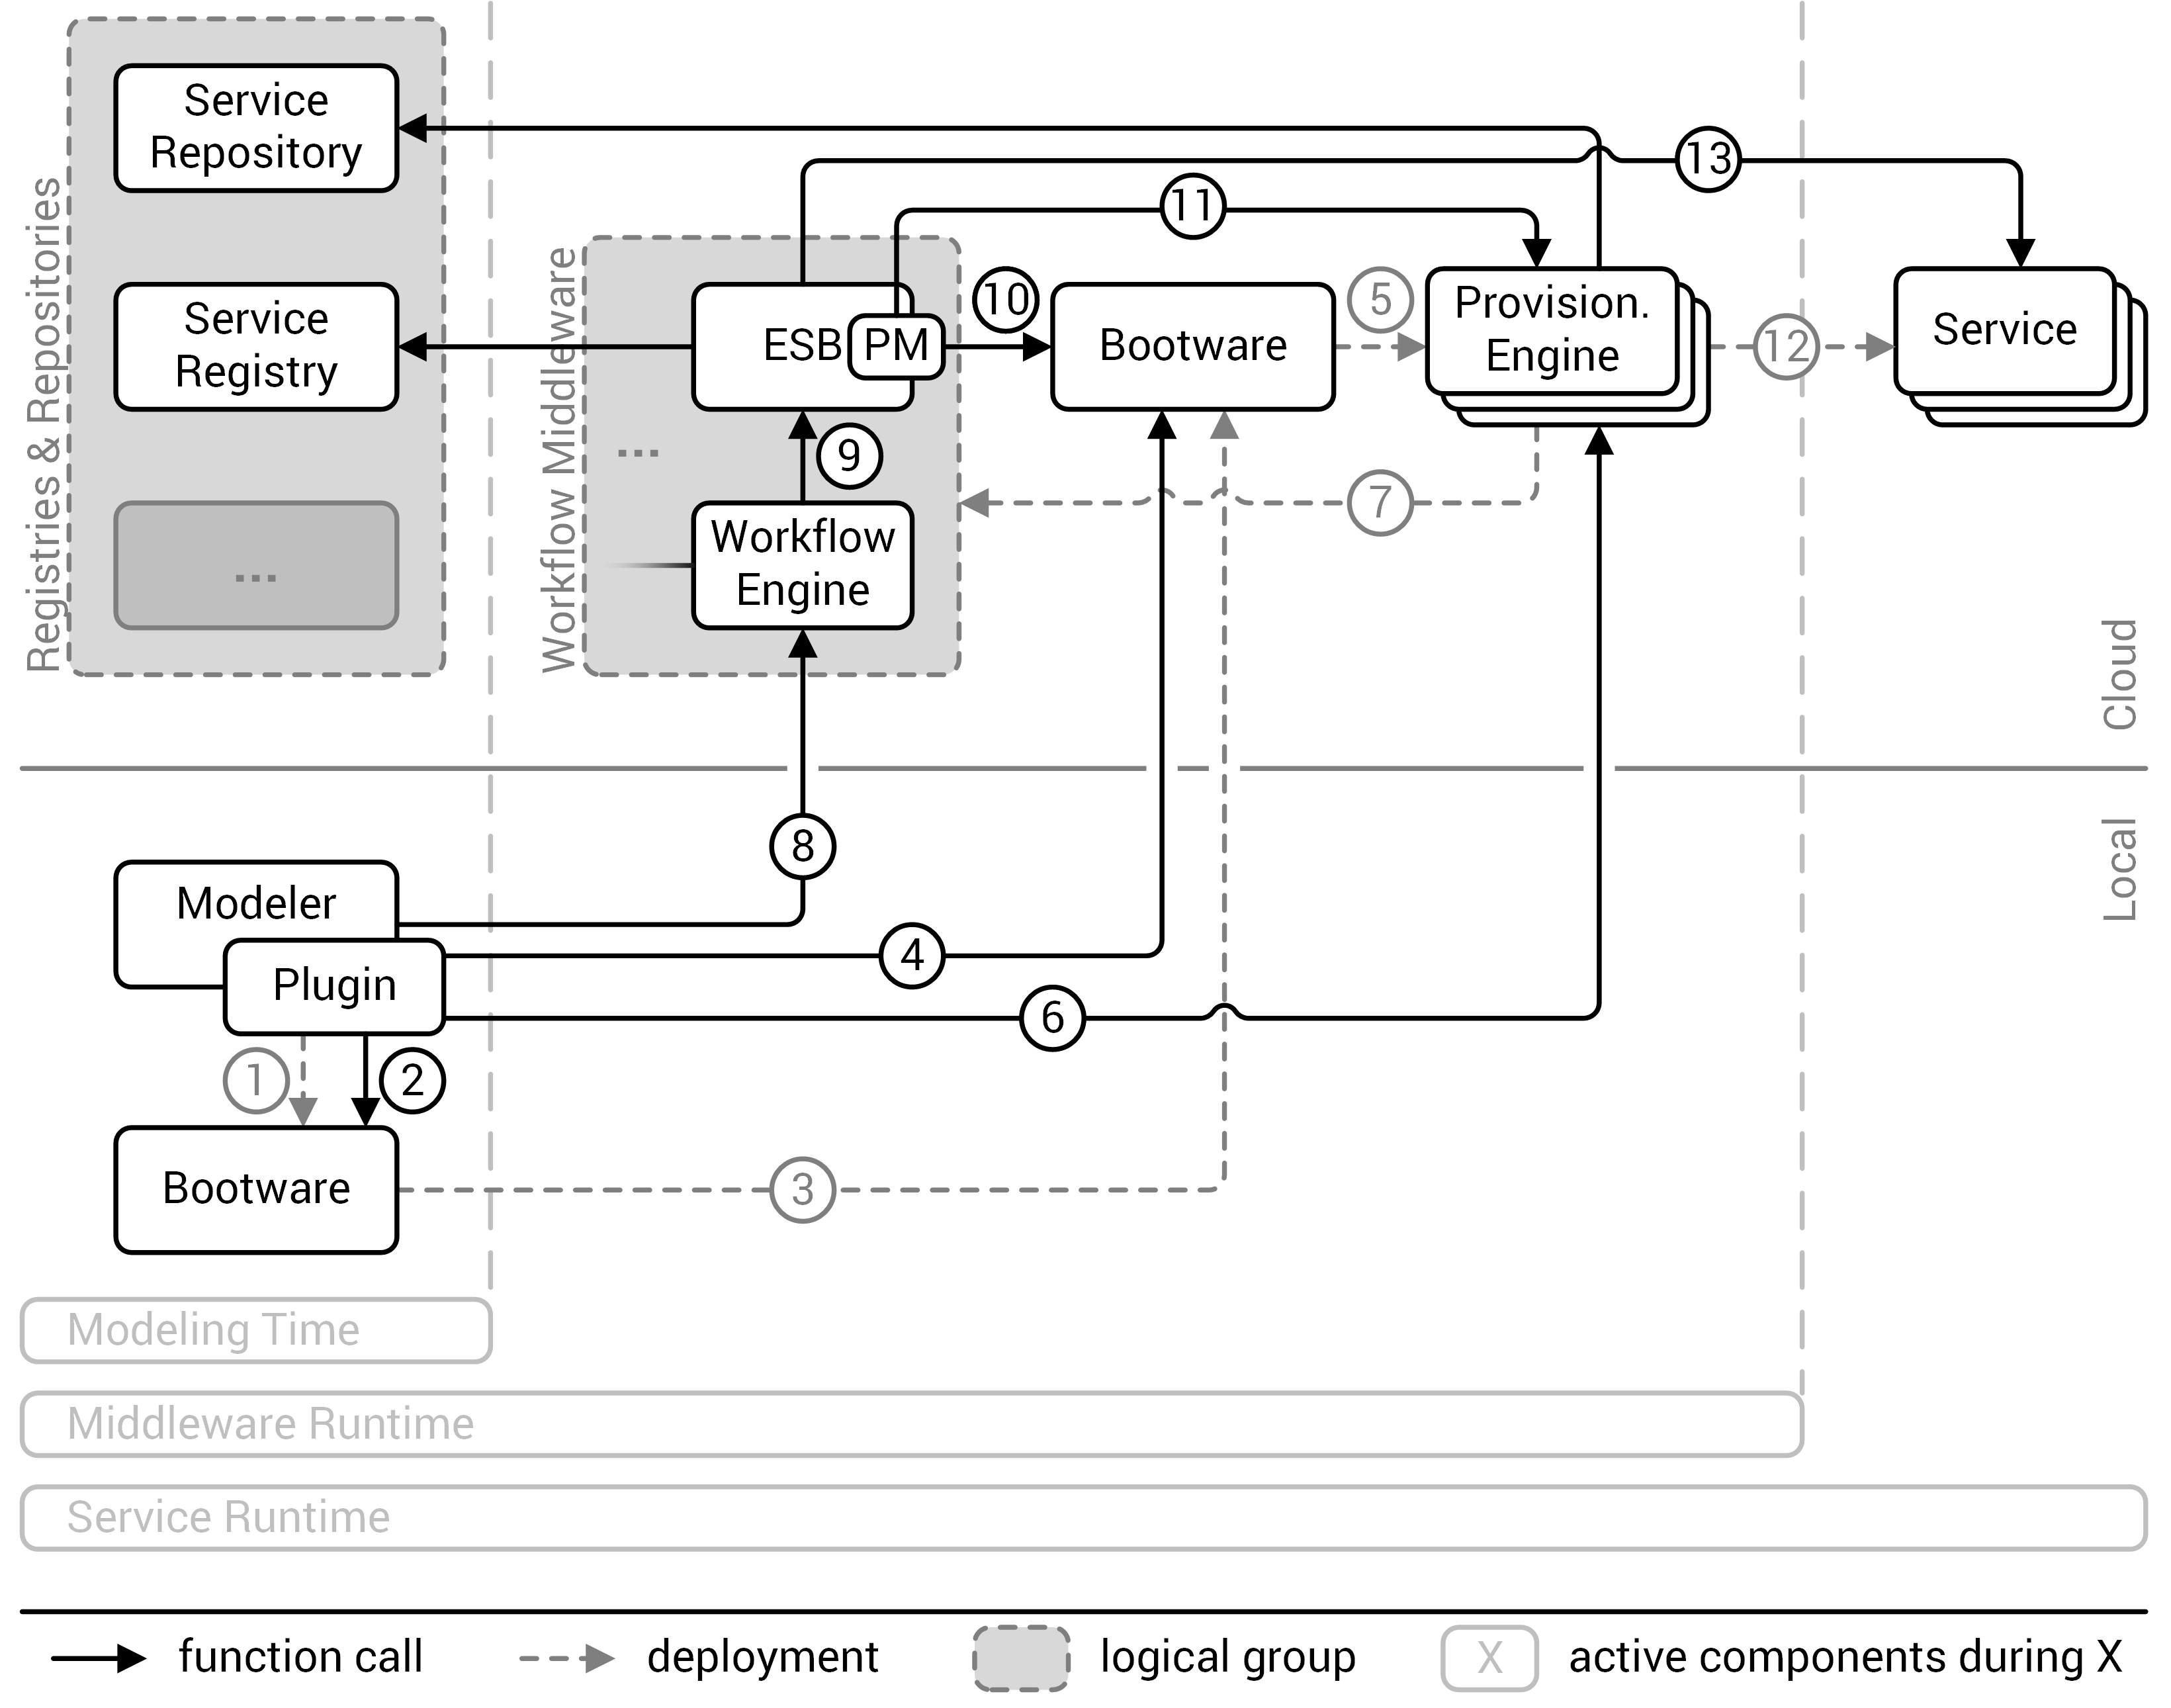
\includegraphics[resolution=600]{process/assets/process}
	\caption{The step-by-step bootware process.}
	\label{image:process}
\end{figure}

At the beginning, a user starts the Modeler, which includes the bootware plugin, as seen on the bottom left of \autoref{image:process}.
If he hasn't done so already, he tells the bootware plugin his cloud login credentials to be used during the bootware process and which event plugins the bootware should load.
He then uses the Modeler to create a workflow as usual.
Once the workflow is finished and ready to be deployed, he clicks the deploy button as usual.
The bootware plugin has hooked into the deploy process and takes over by starting the local bootware (step 1).

Once the local bootware is up and running, the bootware plugin calls it with the context the user provided (step 2).
The local bootware first checks, if a remote bootware already exists in the requested remote environment.
If not, the local bootware provisions a remote bootware using the information provided in the context (step 3).
Once the remote bootware is deployed, it is called by the local bootware with a deploy request for the provisioning engine that will be used to deploy the SimTech SWfMS (step 4).
The remote bootware deploys the requested provisioning engine using the information provided in the context (step 5).
Once the provisioning engine is up and running, the remote bootware calls the provisioning engine (step 6) and tells it to deploy the SimTech SWfMS (step 7).
Once the SimTech SWfMS is up and running, the provisioning engine returns the endpoint references of the SimTech SWfMS to the remote bootware, which in turn returns it to the local bootware, which returns it to the bootware pluhin.
The bootware plugin uses these end point references to link the modeler to the SimTech SWfMS.

Once linked, the modeler deploys the workflow on the SimTech SWfMS as usual and starts its execution (step 8).
The SimTech SWfMS now executes the workflow, during which it might encounter a point where it has to call a remote service.
The remote service call is passed on to the ESB (step 9), which checks if the service is already reachable.
If it is, execution continues as usual.
If not, the ESB tells the provisioning manager to provision the requested service (step 10).
The provisioning manager checks, if the provisioning engine needed to provision the requested service is already available.
If it isn't, the provisioning manager calls the remote bootware with a request to provision the required provisioning engine (step 11).
The remote bootware provisions the provisioning engine using the information from the request and the user context (step 5).
Once the provisioning engine is up and running, the remote bootware returns a endpoint reference to the provisioning manager.
The provisioning manager now calls the provisioning engine (step 12) and tells it to provision the required service (step 13).
Once the service is available, the provisioning engine returns its endpoint reference to the provisioning manager, who in turn returns it to the ESB.
The ESB can now call the service (step 14) and use the service response to continue with the workflow execution.

The workflow execution now continues in this fashion, spawning new provisioning engines and services through the provisioning manager and the remote bootware along the way (repeating steps 10, 11, 5, 12, 13 and 14).
At some point, the workflow will be finished.
If it hasn't done so already, the provisioning manager calls all relevant provisioning engines to undeploy any services that might still be running (step 12, 13).
Once all services are undeployed, the work of the SimTech SWfMS is finished.
The bootware is listening at the SimTech SWfMS for this event and triggers the undeploy process once it happens.
First, the remote bootware calls the provisioning engine that was used to provision the SimTech SWfMS (step 6) and tells it to undeploy the SimTech SWfMS (step 7).
The provisioning engine returns the success to the remote bootware.
Next, the remote bootware undeploys all provisioning engines that might still be running (step 5).
Once all provisioning engines are gone, the remote bootware returns the success to the local bootware.
The local bootware removes the remote bootware (step 3) and returns the success to the bootware plugin.
At this point, no remote components should be running anymore.
The bootware plugin now tells the local bootware to shutdown (step 1), which completes the whole process.

\begin{figure}[!htbp]
	\centering
	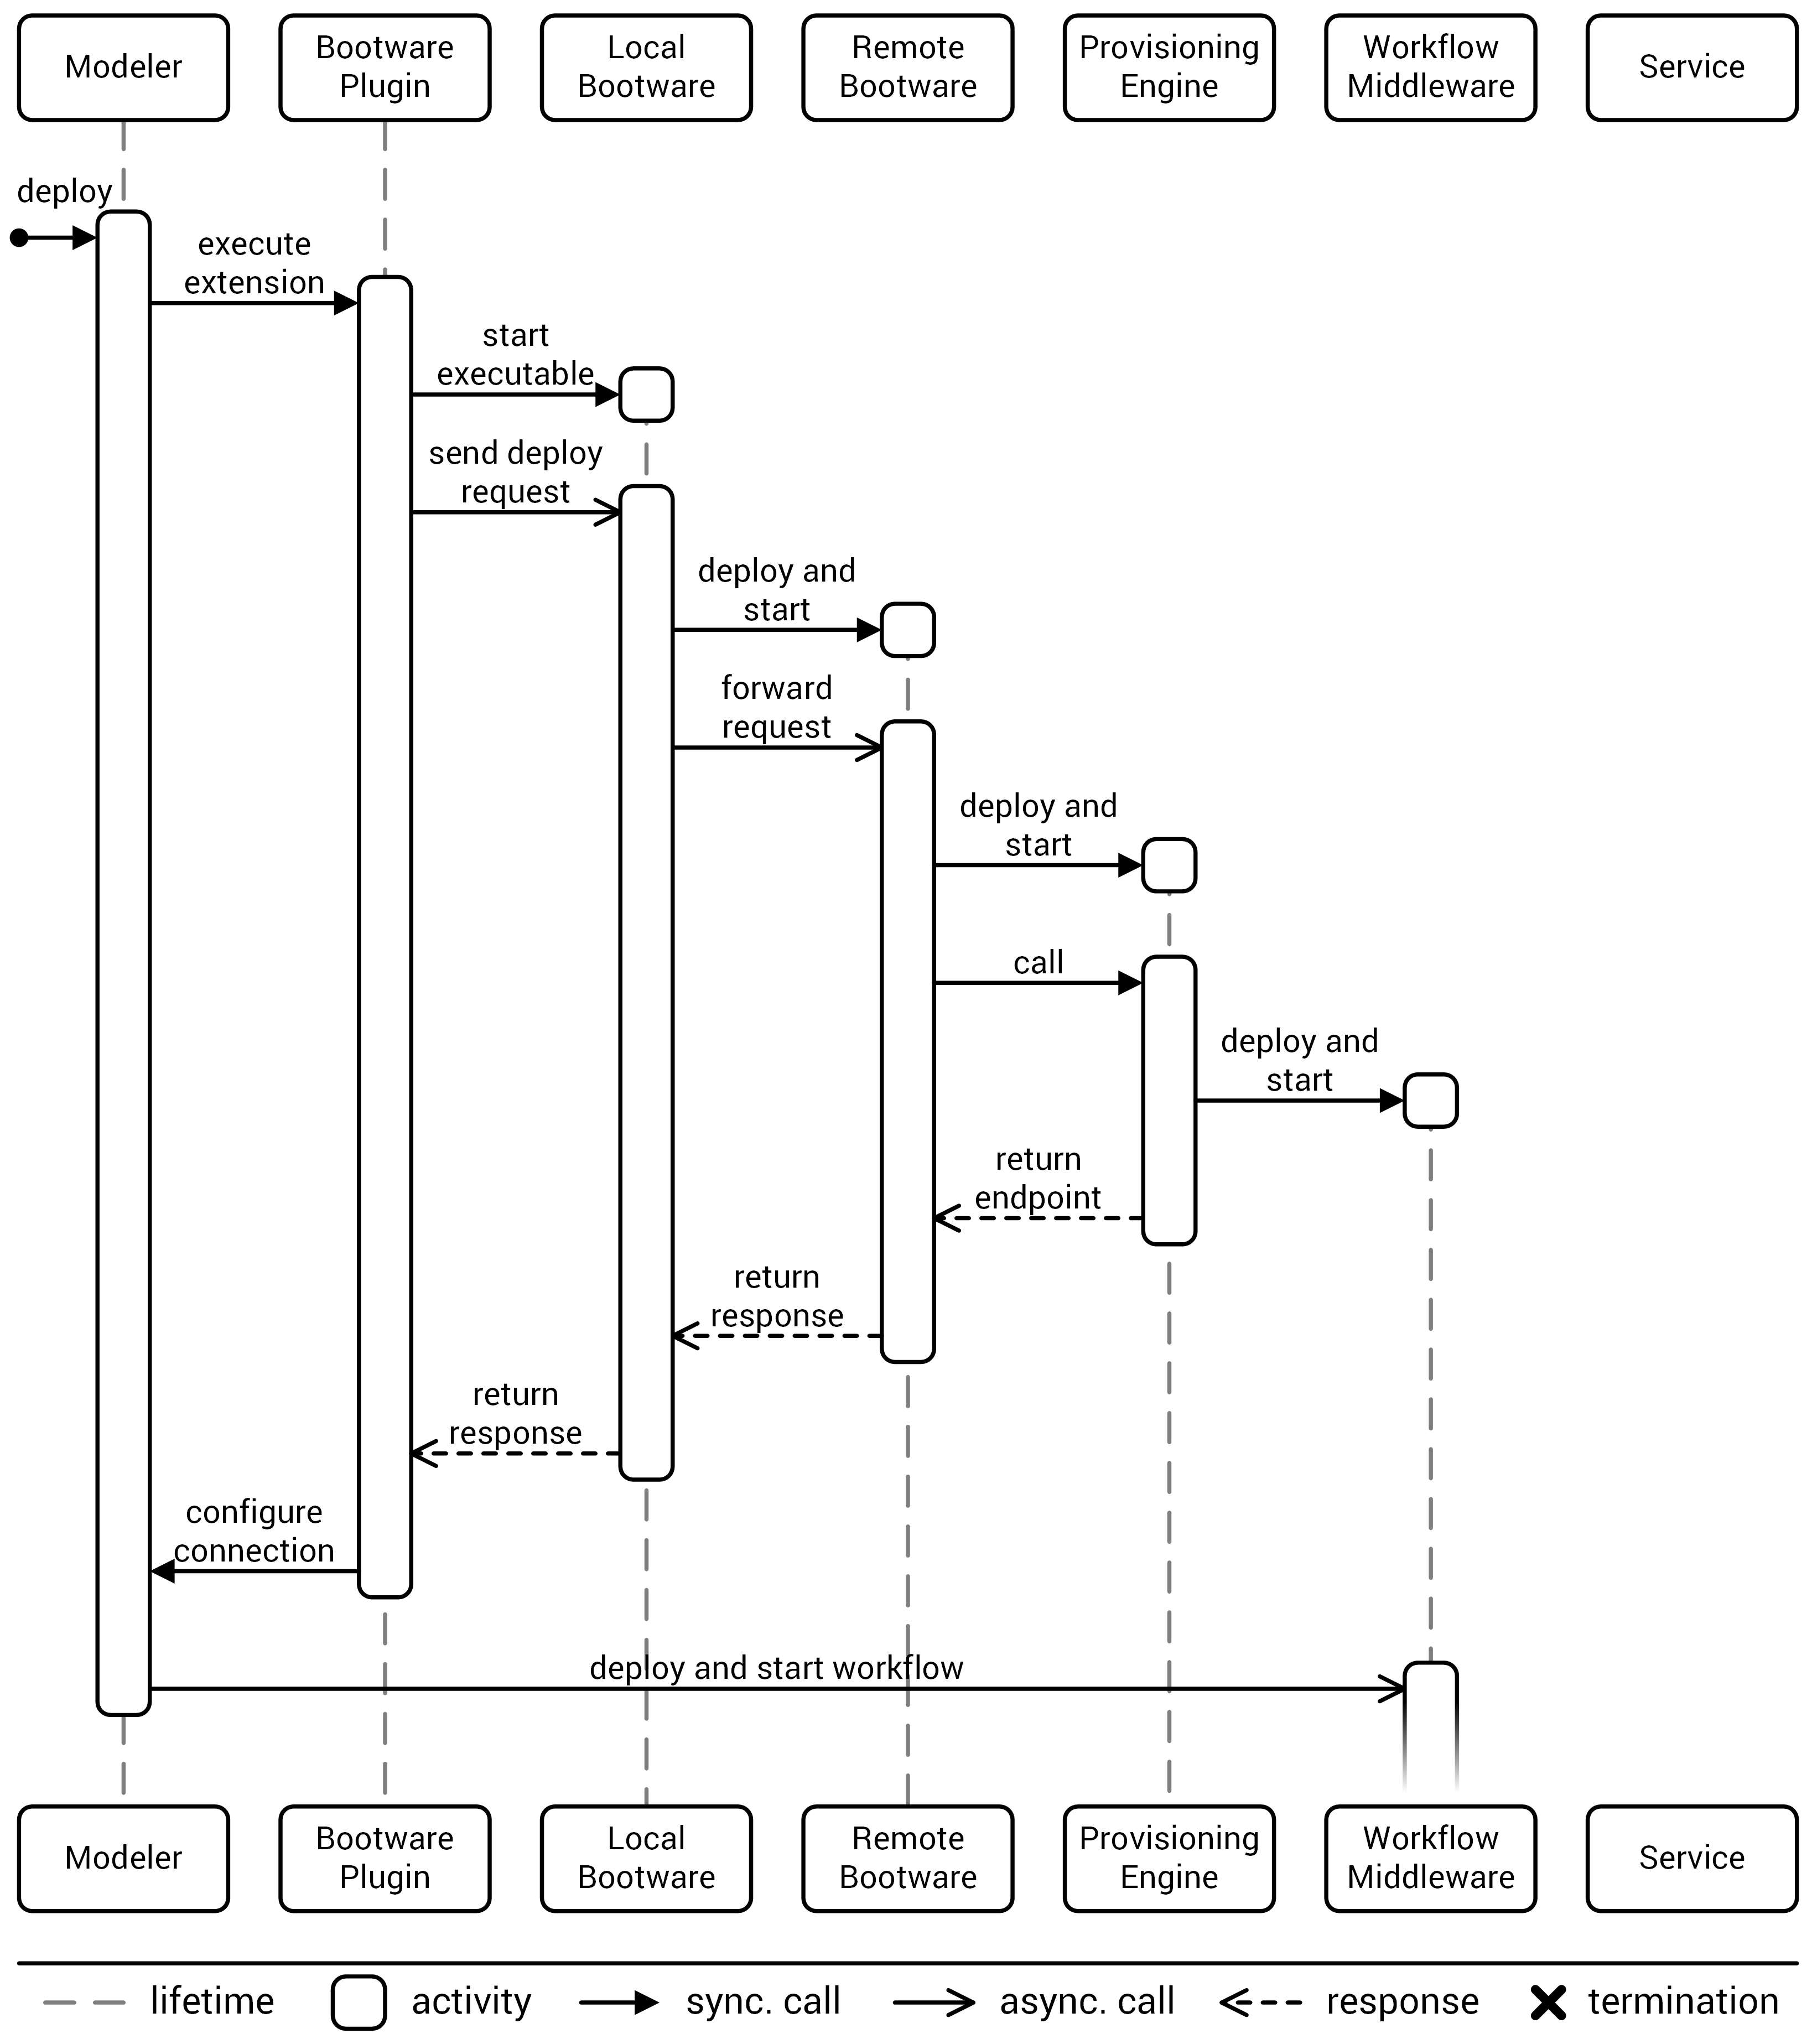
\includegraphics[resolution=600]{process/assets/bootstrapping_sequence}
	\caption{Sequence diagram of the bootstrapping phase.}
	\label{image:startup_sequence}
\end{figure}

\begin{figure}[!htbp]
	\centering
	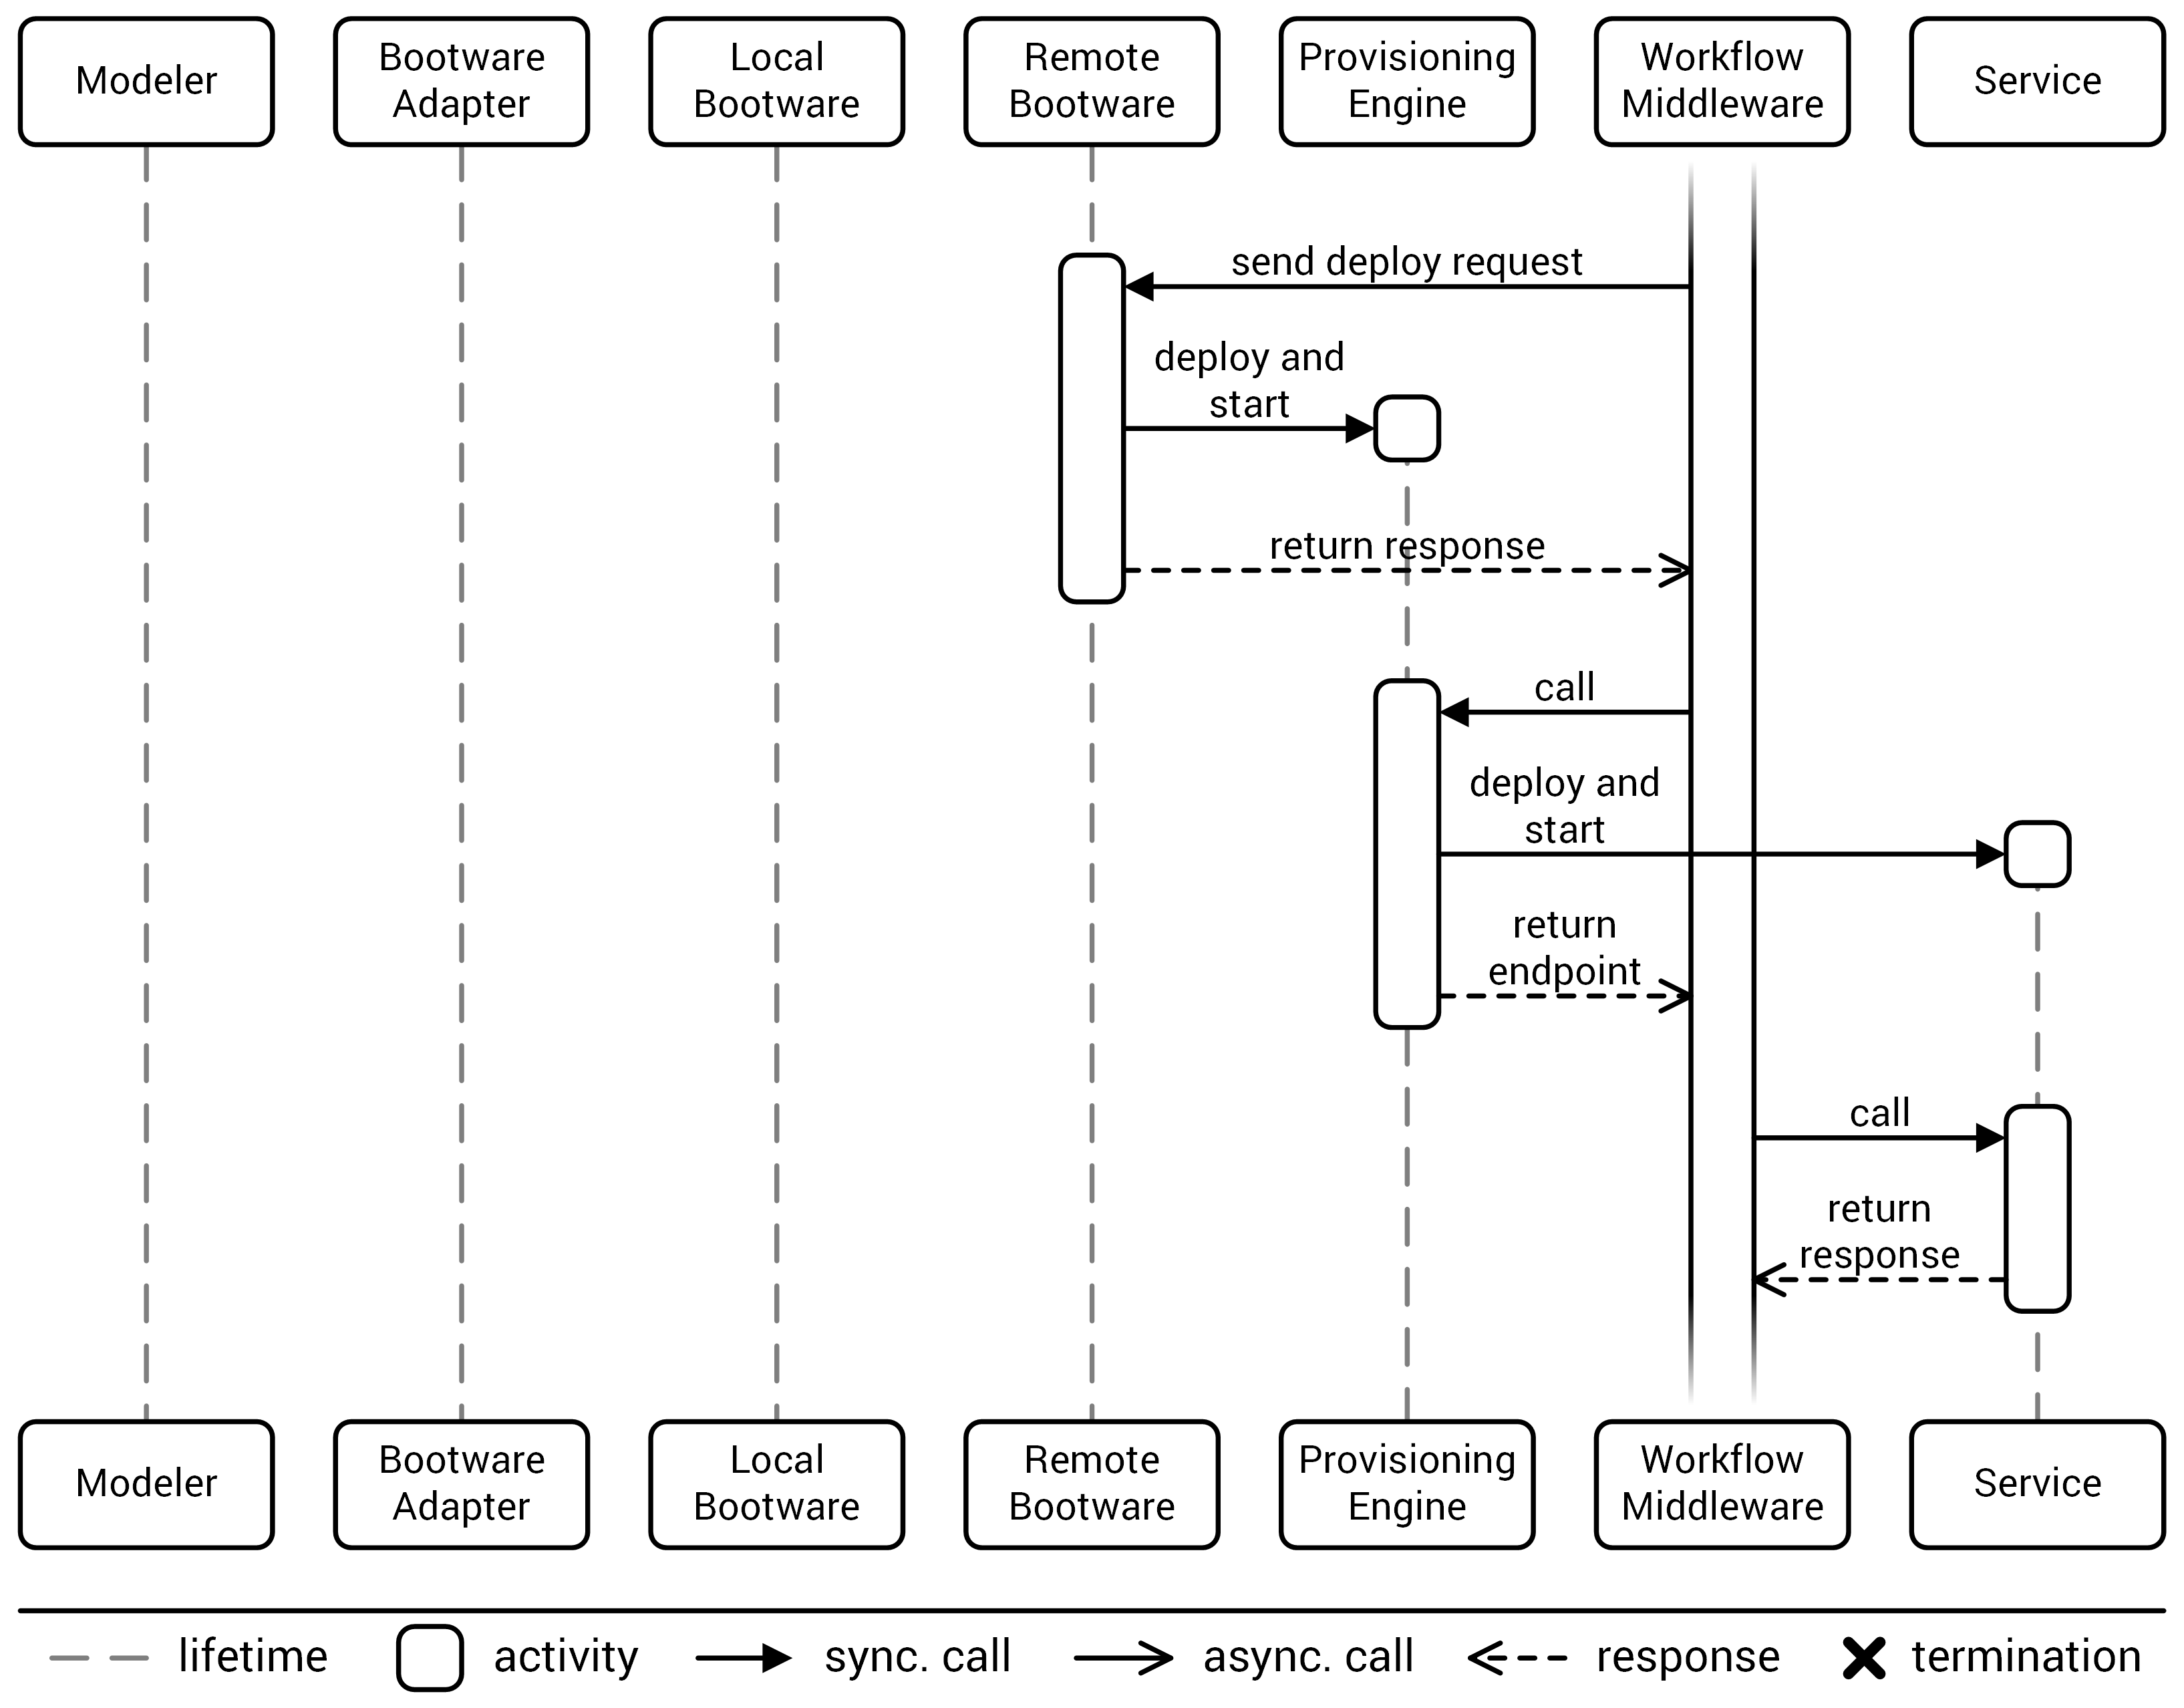
\includegraphics[resolution=600]{process/assets/workflow_execution_sequence}
	\caption{Sequence diagram of the workflow execution phase.}
	\label{image:execution_sequence}
\end{figure}
